\documentclass{article}

\textwidth=6.5in
\textheight=8.5in
\voffset=-54pt
\oddsidemargin=0in
\evensidemargin=0in
\setlength{\parskip}{8pt}
\setlength{\parindent}{0pt}

\usepackage{amsmath, amssymb}
\usepackage{ifthen}

\usepackage[inline]{enumitem}
\setlist{topsep=0pt, parsep=8pt}

\usepackage[rgb,table]{xcolor}\convertcolorsUfalse
\usepackage{graphicx}

% change hyperref options
\PassOptionsToPackage{hyphens}{url}
\usepackage[bookmarks,colorlinks,linkcolor=black,citecolor=blue,pdfstartview=FitH,urlcolor=blue]{hyperref}
\hypersetup{pdfpagemode=UseNone}
\usepackage{bookmark}

\usepackage{graphicx}
\usepackage{multicol}
\usepackage{framed}
\usepackage{array}

\usepackage{icomma}

\usepackage{soul}
\usepackage[normalem]{ulem}

\usepackage{pgfplots}
\pgfplotsset{compat=1.18}  
\pgfplotscreateplotcyclelist{mycolor}{black, blue, red, green!70!black, magenta, purple, cyan, orange }  
\pgfplotsset{
  disabledatascaling,
  cycle list=tikzcolor, 
  axis lines=middle,
  every axis plot/.style={no marks, thick},
  every axis/.style={
    enlarge x limits=false,
    enlarge y limits=auto,
    xlabel style={at={(current axis.right of origin)},anchor=west},
    ylabel style={at={(current axis.above origin)},anchor=south},
    % extra x and y ticks for asymptotes
    extra x tick style={grid=major, grid style={dashed,black}},
    extra y tick style={grid=major, grid style={dashed,black}},
    /pgf/number format/1000 sep={},
  },    
  tick label style = {font=\footnotesize, fill=\currentbgcolor, inner sep=0pt},    
  xticklabel shift=1pt,    
  scaled ticks=false,
  scaled y ticks=false,
  unbounded coords=jump,
  samples=101,
  minor tick length=0,
  scatter/classes={
    open={mark=*,draw=black,fill=white, mark size=2, thin},
    closed={mark=*,draw=black,fill=black, mark size=2, thin}
  },
  width=3in,
}
\pgfplotsset{open/.style={only marks, mark=*, fill=white, thin, mark size=2}}
\pgfplotsset{closed/.style={only marks, mark=*, draw=black, fill=black,
    thin, mark size=2}}
\pgfplotsset{labeled/.style={nodes near coords, only marks, mark=*, draw=black, fill=black, thin, mark size=2, point meta=explicit symbolic}}

\pgfplotsset{gridgraph/.style={clip=false, axis line style={shorten
      >=-8pt}, xlabel style={xshift=8pt}, ylabel style={yshift=8pt},
    enlargelimits=false, grid=major, tick style={black}}} 


\usepackage{tikz}
\usetikzlibrary{
  matrix,%
  % enables the snake paths
  decorations.pathmorphing,%
  % enables bigger arrows
  decorations.markings,%
  decorations.pathreplacing,%
  decorations.text,%
  calc,%
  patterns,%
  shapes.geometric,%
  arrows,
  decorations.shapes,
  positioning,
  plotmarks,
  intersections
}
\tikzset{>=latex} % sets default arrow type in tikz
\tikzset{font=\normalsize}
\tikzset{mark size=1.5pt, mark options=thin}
\tikzset{pin distance=4pt,
  every pin edge/.style={<-, thin, shorten <= -2pt}}

\interfootnotelinepenalty=10000
\renewcommand{\thefootnote}{(\arabic{footnote})}

\usepackage{multirow, bigdelim}

% change to \usepackage[sols]{handout} to see solutions
\usepackage[sols]{handout}

\newcommand\iscurrentenumi[1]{%
  \ifthenelse{\equal{#1}{\theenumi}}{}{#1}}
\setenumerate[1]{ref=\#\arabic*}
\setenumerate[2]{ref=\protect\iscurrentenumi{\theenumi}(\alph*)}
\newcommand\enumiiprefix[2]{%
  \ifthenelse{{\equal{#1}{\theenumi}}\AND{\equal{#2}{(\alph{enumii})}}}{}{}%
  \ifthenelse{{\equal{#1}{\theenumi}}\AND{\NOT{\equal{#2}{(\alph{enumii})}}}}{#2}{}%
  \ifthenelse{\equal{#1}{\theenumi}}{}{#1#2}%
}
\setenumerate[3]{ref=\protect\enumiiprefix{\theenumi}{(\alph{enumii})}\roman*}

\makeatletter

% underline links               
\let\@href=\href
\renewcommand{\href}[2]{\@href{#1}{\ul{#2}}}

\newdimen\SOUL@dimen %new
\def\SOUL@ulunderline#1{{%
    \setbox\z@\hbox{#1}%
    % \dimen@=\wd\z@
    \SOUL@dimen=\wd\z@ %new
    \dimen@i=\SOUL@uloverlap
    \advance\SOUL@dimen2\dimen@i %\dimen@ exchanged too
    \rlap{%
      \null
      \kern-\dimen@i
      % \SOUL@ulcolor{\SOUL@ulleaders\hskip\dimen@}%
      \SOUL@ulcolor{\SOUL@ulleaders\hskip\SOUL@dimen}% new
    }%
    \unhcopy\z@
  }}

\newcommand\calculator{
  \begin{tikzpicture}[x=0.15ex, y=0.15ex, baseline=1.5pt]
    \begin{scope}[thick]
      \draw (0, 0) -- (10, 0) -- (10, 14) -- (0, 14) -- cycle;
      \foreach \x in {10/3, 20/3}
      {
        \draw (\x, 0) -- (\x, 10);
      }
      \foreach \y in {10/3, 20/3, 10}
      {
        \draw (0, \y) -- (10, \y);
      }
    \end{scope}
  \end{tikzpicture}
}
\newcommand{\calcitem}{\refstepcounter{enum\romannumeral\@enumdepth}%
\item[\calculator \csname labelenum\romannumeral\@enumdepth\endcsname]}

\makeatother

\definecolor{purple}{rgb}{0.5,0,1.0}

\newcommand{\doedfinity}[2][\newpage]{
  \begin{problem}[#1]
    Do the Edfinity assignment ``Problem Set #2''.

    We encourage you to write down any scratch work here, as well as
    things you want your future self to remember. Nothing you write
    here will be graded; it's just for you!
  \end{problem}
}

\newcommand{\psrnewpage}{\newpage}
\newcommand{\psreflection}[2][]{

  \ifthenelse{\not\equal{#1}{nocite}}{
    \begin{enumerate}[resume]
    \item
      \begin{problem}[1in]
        Please cite any help you got on this problem set:
        \begin{itemize}[nosep]
        \item If you worked with other students, please list their names here.
        \item If you used resources other than those on our Canvas site, please list them here.
        \end{itemize}
      \end{problem}

    \end{enumerate}
  }

  \probonly{%
    #2

    \psrnewpage

    \emph{Reflection space.} It's a good habit to take a few minutes at the end of each pset to reflect on what you learned and jot down notes to your future self. Here are a few reflection questions to get you started. Nothing you write here will be graded; it's just for you!
    \begin{itemize}
    \item Take a few minutes to look back at the problems. How could you explain to someone else how to do each problem? What was your strategy, and how did you know to use that strategy? If there are problems where you don't feel able to answer this, write down which ones they are. Come back to them in a few days when we post the homework solutions!

      \vspace{1.5in}

    \item Take a look back at the learning objectives on today's worksheet; how are you feeling about each one? If there are ones you know you need more practice with, write those down here.

      \vspace{1.5in}

    \item What did you find most challenging about this material? Do you have any lingering questions about it? If so, write them down here so you don't forget them. At some point, stop by office hours or MQC to ask!

      \vfill
    \end{itemize}      
  }
}

\usepackage{fancyhdr}
\lhead{\textcolor{white}{This content is protected and may not be shared, uploaded, or distributed.}}
\rhead{}
\rfoot{\vspace*{\fill}\footnotesize\textcopyright{} \emph{Harvard Math Ma}}
\renewcommand{\headrulewidth}{0pt}
\pagestyle{fancy}
\begin{document}

\begin{center}
  \large\textsc{Problem Set 12 - Using Derivatives to Graph Functions}\vspace{.5in}\\
  \begin{problemonly}
   \large Name: \rule{5cm}{0.15mm}\\
   \end{problemonly}
\end{center}

\begin{enumerate}
\item  \note{
    \begin{itemize}[nosep]
    \item Given formula for $f'$, identify turning points of $f$.
    \item Given formula for $f''$, identify inflection points of $f$.
    \item Given graph of $f'$, identify where $f$ is concave down. 
    \item Order quantities like $\dfrac{0.01}{0.00001}$, $\dfrac{0.00001}{0.01}$, etc. (preparation for limits)
    \end{itemize}
  }

  \doedfinity{12}

\item \label{deriv-of-ax^3+bx}

  \begin{grading} 
    4 points:
    \begin{itemize}[nosep]
    \item 3 for correctly simplifying the difference quotient $\dfrac{ g(x+h) - g(x) }{h}$ (give partial credit if the simplification is partially correct)
    \item 0.5 for using limit notation correctly (writing $\displaystyle \lim_{h \to 0}$ on each line until they actually take the limit)
    \item 0.5 for correct limit
    \item Please call special attention to use of parentheses.
    \end{itemize}
  \end{grading} 

  \begin{problem}[\vfill]
    Let $g(x) = ax^3 + bx$, where $a$ and $b$ are constants. Use the definition of the derivative to calculate $g'(x)$. 
  \end{problem}

  \begin{solution}
    Let's start by writing the definition of the derivative.
    \begin{align*}
      g'(x) &= \lim_{h \to 0} \frac{g(x+h) - g(x)}{h} \\
      &= \lim_{h \to 0} \frac{a(x+h)^3 + b(x+h) - (ax^3+bx)}{h} \\
      \intertext{Now we can expand and simplify.}
      &= \lim_{h \to 0} \frac{a(x+h)^2(x+h) + b(x+h) - (ax^3+bx)}{h} \\
      &= \lim_{h \to 0} \frac{a(x^2+2xh+h^2)(x+h) + b(x+h) - (ax^3+bx)}{h} \\
      &= \lim_{h \to 0} \frac{a(x^3+3x^2h+3xh^2+h^3) + b(x+h) - (ax^3+bx)}{h} \\
      &= \lim_{h \to 0} \frac{ax^3+3ax^2h+3axh^2+ah^3 + bx+bh - ax^3-bx}{h} \\
      &= \lim_{h \to 0} \frac{3ax^2h+3axh^2+ah^3 + bh}{h} \\
      \intertext{Now we can factor and cancel $h$.}
      &= \lim_{h \to 0} \frac{h(3ax^2+3axh+ah^2 + b)}{h} \\
      &= \lim_{h \to 0} (3ax^2+3axh+ah^2 + b) \\
      \intertext{Now we use direct substitution to evaluate the limit.}
      &= 3ax^2+3ax(0)+a(0)^2 + b \\
      &= \boxed{3ax^2 + b}
    \end{align*}
  \end{solution}

\item \label{sketch-from-cubic-derivative-1}
  We have the following information about an unknown function $f(x)$:
  \begin{itemize}[nosep]
  \item $f$ is continuous on $(-\infty, \infty)$.
  \item $f$ is even.
  \item $f'(x) = 12x - x^3$.
  \end{itemize}

  \begin{enumerate}
  \item \label{sketch-from-cubic-derivative-1-increase-decrease}

    \begin{grading}
      3 points: 0.5 for correct intervals of increase / decrease, 0.5 for identifying the correct turning points, 2 for a correct approach like making a sign chart 
    \end{grading}

    \begin{problem}[\nstretch{0.4}]
      Where is $f$ increasing? Where is $f$ decreasing? What are its turning points?
    \end{problem}

    \begin{solution}
      Let's make a sign chart for $f'(x)$. We'll do it using algebra. First, we need to find where $f'(x)$
      is zero or undefined. We can see that $f'(x)$ is never undefined. Let's solve $f'(x)=0$.
      \begin{align*}
        -x^3+12x &= 0 \\
        -x(x^2-12) &= 0 \\
        -x(x-\sqrt{12})(x+\sqrt{12}) &= 0
      \end{align*}
      We can see from here that $f'(x)$ is zero when $x=0$ and when $x=\pm \sqrt{12}=\pm 2\sqrt{3}$.

      We can put these values on our sign chart.
      \begin{center}
        \begin{tikzpicture}
          \draw[<->] (-2,0) -- (2,0);
          \node[left] at (-2,0) {$f'(x)$};
          \foreach \x in {-1,0,1}
            \draw[shift={(\x,0)},color=black] (0pt,3pt) -- (0pt,-3pt);
          \node[below] at (-1,-0.1) {$-2\sqrt{3}$};
          \node[below] at (0,-0.1) {$0$};
          \node[below] at (1,-0.1) {$2\sqrt{3}$};
          \foreach \x in {-1, 0, 1}
            \node[circle, fill=black, inner sep=2pt] at (\x,0) {};
        \end{tikzpicture}
      \end{center}

      Now we need to test the value of $f'(x)$ at one $x$-value in each interval.
      \begin{alignat*}{3}
        f'(-4) &= 12(-4)-(-4)^3 &= -48 + 64 &= +16\\
        f'(-1)  &= 12(-1) - (-1)^3   &= -12 + 1 &= -11 \\
        f'(1)  &= 12(1) - (1)^3  &= 12-1 &= +11 \\
        f'(-4) &= 12(4)-(4)^3 &= 48 - 64 &= -16\\
      \end{alignat*}
      We can use this information to complete our sign chart.
      \begin{center}
        \begin{tikzpicture}
          \draw[<->] (-2,0) -- (2,0);
          \node[left] at (-2,0) {$f'(x)$};
          \foreach \x in {-1,0,1}
            \draw[shift={(\x,0)},color=black] (0pt,3pt) -- (0pt,-3pt);
          \node[below] at (-1,-0.1) {$-2\sqrt{3}$};
          \node[below] at (0,-0.1) {$0$};
          \node[below] at (1,-0.1) {$2\sqrt{3}$};
          \foreach \x in {-1, 0, 1}
            \node[circle, fill=black, inner sep=2pt] at (\x,0) {};
          \node[above] at (-1.5,0) {$+$};
          \node[above] at (-0.5,0) {$-$};
          \node[above] at (0.5,0) {$+$};
          \node[above] at (1.5,0) {$-$};
        \end{tikzpicture}
      \end{center}
      
      From this sign chart, we can conclude:
      \begin{itemize}
        \item $f$ is increasing on $(-\infty, -2\sqrt{3})$ and on $(0, 2\sqrt{3})$
        \item $f$ is decreasing on $(-2\sqrt{3}, 0)$ and on $(2\sqrt{3}, \infty)$
        \item $f$ has turning points at $x=0$ and $x=\pm 2\sqrt{3}$
      \end{itemize}
    \end{solution}

  \item

    \begin{grading}
      1 point
    \end{grading}

    \begin{problem}[\stretch{0.25}]
      Use \ref{deriv-of-ax^3+bx} to calculate $f''(x)$.
    \end{problem}

    \begin{solution}
      Since $f''$ is the derivative of $f'$, we can use our formula that $\frac{d}{dx}(ax^3+bx)=3ax^2+b$ 
      to determine that $f''(x) = -3x^2 + 12$. 
    \end{solution}

  \item

    \begin{grading}
      3 points, same breakdown as (a)
    \end{grading}

    \begin{problem}[\vfill]
      Where is $f$ concave up? Where is $f$ concave down? What are its inflection points? 
    \end{problem}

    \begin{solution}
      Let's make a sign chart for $f''(x)$. We'll do it by sketching a rough graph. We know that the graph
      of $y=-3x^2+12$ will be a parabola that opens downwards. To find the $x$-intercepts, we can factor:
      \begin{align*}
          y &= -3x^2 + 12\\
          &= -3(x^2-4)\\
          &= -3(x+2)(x-2)
      \end{align*}
      From here, we can see that the $x$-intercepts are $\pm 2$. So the graph looks like this.  
       \begin{center}
        \begin{tikzpicture}
          \draw[<->] (-4,0) -- (4,0);
          \draw[domain=-4:4, variable=\x, smooth] plot ({\x}, {(-3*\x*\x + 12)/30});
          \node[left] at (-4,-1) {$f''(x)$};
          \foreach \x in {-2,2}
            \draw[shift={(\x,0)},color=black] (0pt,3pt) -- (0pt,-3pt) node[below] {$\x$};
          \foreach \x in {-2, 2}
            \node[circle, fill=black, inner sep=2pt] at (\x,0) {};
        \end{tikzpicture}
      \end{center}

      We can produce the following sign chart.
       \begin{center}
        \begin{tikzpicture}
          \draw[<->] (-4,0) -- (4,0);
          \node[left] at (-4,0) {$f''(x)$};
          \foreach \x in {-2,2}
            \draw[shift={(\x,0)},color=black] (0pt,3pt) -- (0pt,-3pt) node[below] {$\x$};
          \foreach \x in {-2, 2}
            \node[circle, fill=black, inner sep=2pt] at (\x,0) {};
          \node[above] at (-3,0) {$-$};
          \node[above] at (0,0) {$+$};
          \node[above] at (3,0) {$-$};
        \end{tikzpicture}
      \end{center}
      
      From this sign chart, we can conclude:
      \begin{itemize}
        \item $f$ is concave up on $(-2,2)$
        \item $f$ is concave down on $(-\infty,-2)$ and on $(2, \infty)$
        \item $f$ has inflection points at $x=\pm \sqrt{12}$
      \end{itemize}
    \end{solution}

  \item \label{sketch-from-cubic-derivative-1-possibility-1}

    \begin{grading}
      4.5 points:
      \begin{itemize}[nosep]
      \item 1 for graph being increasing and concave up on $(0, 2)$
      \item 1 for increasing and concave down on $(2, 2 \sqrt{3})$
      \item 1 for decreasing and concave down on $(2 \sqrt{3}, \infty)$
      \item 1 for symmetry over $y$-axis
      \item 0.5 for $f(0) = 5$
      \end{itemize}
    \end{grading}

    \begin{problem}[\stretch{2}]
      If $f(0) = 5$, sketch a possible graph of $f$. Please label the $x$-axis with the values of all turning points and inflection points. Your graph should be consistent with the given information, as well as what you've figured out so far. 
    \end{problem}

    \begin{solution}
      First, let's sketch a graph that's consistent with the information we found in part (a). We know
      $f$ should be decreasing on $(-2\sqrt{3}, 0)$ and on $(2\sqrt{3}, \infty)$
      and increasing on $(-\infty, -2\sqrt{3})$ and on $(0, 2\sqrt{3})$. 
      There should be horizontal tangents at the turning point, but we'll smooth them out later.

      \begin{center}
        \begin{tikzpicture}
          \begin{axis}[ytick={5}, xtick={-3.46, 3.46}, xticklabels={$-2\sqrt{3}$, $2\sqrt{3}$}]
            \addplot+[domain=-5.5:-3.46, dashed] {25*x+126.1};
            \addplot+[domain=-3.46:0, dashed] {-10*x+5};
            \addplot+[domain=0:3.46, dashed] {10*x+5};
            \addplot+[domain=3.46:5.5, dashed] {-25*x+126.1};
          \end{axis}
        \end{tikzpicture}
      \end{center}

     Note that we're told that that $f(0)=5$, but don't know where the $x$-intercepts actually are.

     Now let's revise our graph to represent the information we found in part (c). We know that $f$ should
     be concave up on $(-\infty, 0)$ and $(0, \infty)$. 
      \begin{center}
        \begin{tikzpicture}
          \begin{axis}[ytick={5}, xtick={-3.46, -2, 2, 3.46}, xticklabels={$-2\sqrt{3}$, $-2$, $2$, $2\sqrt{3}$}]
            \addplot+[domain=-5.5:5.5] {-x^4/4 + 6*x^2 +5};
          \end{axis}
        \end{tikzpicture}
      \end{center}
      
    \end{solution}

  \item

    \begin{grading}
      2 points: 1 for sketching a vertical shift with $y$-intercept of $-5$, 1 for saying it's a vertical shift
    \end{grading}

    \begin{problem}[\nstretch{2}]
      If $f(0) = -5$, sketch a possible graph of $f$. How does it relate to the graph you sketched in \ref{sketch-from-cubic-derivative-1-possibility-1}? 
    \end{problem}

    \begin{solution}
      If we're told $f(0)=-5$ instead of $f(0)=5$, then the intervals on which $f$ is increasing/decreasing and
      concave up/concave down won't change, but the graph will be shifted downwards by 10 units.
      \begin{center}
        \begin{tikzpicture}
          \begin{axis}[ytick={-5}, xtick={-3.46, -2, 2, 3.46}, xticklabels={$-2\sqrt{3}$, $-2$, $2$, $2\sqrt{3}$}]
            \addplot+[domain=-5.5:5.5] {-x^4/4 + 6*x^2 -5};
          \end{axis}
        \end{tikzpicture}
      \end{center}
    \end{solution}

  \end{enumerate}

\item  In this problem, both \ref{deriv-of-ax^3+bx} and \href{https://canvas.harvard.edu/files/20768202/download?download_frd=1}{Problem Set 10}, {{{{\#3}}(a)}} will be useful.

  Let $f(x) = 3x^3 + x$.
  \begin{enumerate}
  \item

    \begin{grading}
      4 points: 1 for calculating $f'$, 3 like \ref{sketch-from-cubic-derivative-1-increase-decrease}
    \end{grading}

    \begin{problem}[\vfill]
      Without using technology, determine where $f$ is increasing and where it's decreasing. Where are its turning points? 
    \end{problem}

    \begin{solution}
      We should make a sign chart for $f'$, but first we need to find $f'(x)$. Using our formula from
      \ref{deriv-of-ax^3+bx}, $\frac{d}{dx}(ax^3+bx)=3ax^2+b$, we know that $f'(x)=9x^2+1$.
      Now, we can sketch a rough graph of $f'$. It will be the graph of $y=x^2$ but scaled vertically and shifted
      upwards. From this, we can tell that there won't be any $x$-intercepts, so the graph looks like this.

      \begin{center}
        \begin{tikzpicture}[xscale=2]
          \draw[<->] (-1,0) -- (1,0);
          \draw[domain=-1:1, variable=\x, smooth] plot ({\x}, {(9*\x*\x + 1)/10});
          \node[left] at (-1,1) {$f'(x)$};
        \end{tikzpicture}
      \end{center}

      This means that we have the following sign chart.

      \begin{center}
        \begin{tikzpicture}[xscale=2]
          \draw[<->] (-1,0) -- (1,0);
          \node[left] at (-1,0) {$f'(x)$};
          \node[above] at (0,0) {$+$};
        \end{tikzpicture}
      \end{center}

      From this sign chart, we can conclude:
      \begin{itemize}
        \item $f$ is increasing on $(-\infty, \infty)$
        \item $f$ is not decreasing on any interval
        \item $f$ has no turning points
      \end{itemize}
      
    \end{solution}

  \item \label{3x^3+x-concavity}

    \begin{grading}
      4 points, same breakdown as (a)
    \end{grading}

    \begin{problem}[\vfill]
      Without using technology, determine where $f$ is concave up and where it's concave down. What are its inflection points?
    \end{problem}

    \begin{solution}
      We should make a sign chart for $f''$, but first we need to find $f''(x)$. Since $f''(x)$ is the derivative
      of $f'(x)=9x^2+1$, using our formula from
      Problem Set 10 \#3(a), $\frac{d}{dx}(ax^2+bx+c)=2ax+b$, we know that $f''(x)=18x$.
      Let's sketch a rough graph of $f''$. The graph
      will be a line with positive slope passing through the origin.

      \begin{center}
        \begin{tikzpicture}[xscale=2]
          \draw[<->] (-1,0) -- (1,0);
          \draw[domain=-1:1, variable=\x, smooth] plot ({\x}, {\x/2});
          \node[left] at (-1,-0.5) {$f''(x)$};
          \foreach \x in {0}
            \draw[shift={(\x,0)},color=black] (0pt,3pt) -- (0pt,-3pt) node[below] {$\x$};
          \foreach \x in {0}
            \node[circle, fill=black, inner sep=2pt] at (\x,0) {};
        \end{tikzpicture}
      \end{center}

      This means that we have the following sign chart.

      \begin{center}
        \begin{tikzpicture}[xscale=2]
          \draw[<->] (-1,0) -- (1,0);
          \node[left] at (-1,0) {$f''(x)$};
          \foreach \x in {0}
            \draw[shift={(\x,0)},color=black] (0pt,3pt) -- (0pt,-3pt) node[below] {$\x$};
          \foreach \x in {0}
            \node[circle, fill=black, inner sep=2pt] at (\x,0) {};
          \node[above] at (-0.5, 0) {$-$};
          \node[above] at (0.5, 0) {$+$};
        \end{tikzpicture}
      \end{center}
      From this sign chart, we can conclude:
      \begin{itemize}
        \item $f$ is concave down on $(-\infty, 0)$
        \item $f$ is concave up on $(0, \infty)$
        \item $f$ has an inflection point at $x=0$
      \end{itemize}
      
    \end{solution}

  \item \label{3x^3+x-tangent-line-at-inflection-point-guess}

    \begin{grading}
      2 points: 1 for filling in the blanks correctly, 1 for guess (any thoughtful guess gets full credit, whether or not it's right)
    \end{grading}

    \begin{problem}[\nstretch{0.5}]
      Fill in the blanks. We've seen that:
      \begin{itemize}
      \item When a graph is concave up, its tangent lines are \probonly{\fitb{1in}{}} 
        \solonly{\fitb{1in}{below}} the graph.
      \item When a graph is concave down, its tangent lines are \probonly{\fitb{1in}{}} 
        \solonly{\fitb{1in}{above}} the graph. 
      \end{itemize}
      Make a guess: How do you think the tangent line at an inflection point should relate to the graph? 
    \end{problem}

    \begin{solution}
      At an inflection point, the tangent line will switch from being above the graph to below the graph or vice
      versa.
    \end{solution}

  \item \label{3x^3+x-tangent-line-at-inflection-point}

    \begin{grading}
      2 points: 1 for the slope, 1 for the equation
    \end{grading}

    \begin{problem}[\vfill]
      In \ref{3x^3+x-concavity}, you should have found that $f(x)$ has exactly one inflection point. Find the tangent line there. 
    \end{problem}

    \begin{solution}
      The inflection point is at $x=0$. To write the equation of a tangent line, we need the slope and a point. 
      The point we know is $(0, f(0))$, which is $(0,0)$. The slope is $f'(0)$, and since $f'(x)=9x^2+1$,
      $f'(0) = 1$. The equation of the tangent line is therefore $y=x$. 
    \end{solution}

  \calcitem

    \begin{grading}
      2 points, 1 for the sketch and 1 for the description. (If they made a correct guess in \ref{3x^3+x-tangent-line-at-inflection-point-guess}, they don't need a description here.) 
    \end{grading}

    \begin{problem}[\vfill\newpage]
      Use \href{https://www.desmos.com/calculator}{Desmos} to graph $f(x)$ together with the tangent line you found in \ref{3x^3+x-tangent-line-at-inflection-point}, and sketch what you see. Does it fit the guess you made in \ref{3x^3+x-tangent-line-at-inflection-point-guess}? If not, describe in words how the tangent line relates to the graph. 
    \end{problem}

    \begin{solution}
      Here's what the graph and the tangent line look like.
      \begin{center}
        \begin{tikzpicture}
          \begin{axis}[xtick=\empty, ytick=\empty]
            \addplot[domain=-1:1] {3*x^3 + x};
            \addplot[domain=-1:1, red] {x};
          \end{axis}
        \end{tikzpicture}
      \end{center}
      At $x=0$, the tangent line switches from being above the graph to below the graph.
    \end{solution}

  \end{enumerate}

\item \label{limit-intro} 

  We've seen that the definition of the derivative involves the idea of a limit. Next class, we'll start a deeper dive into the idea of a limit. To prepare, please read \href{https://canvas.harvard.edu/files/20608916/download?download_frd=1}{the ``A Brief Introduction to Limits'' handout}, and then do the following problem.

  Let $f(x) = \dfrac{x^2 - 3x + 2}{(x^2 - x)(x^2 - 2x)}$. In this problem, you'll investigate $\displaystyle \lim_{x \to 2} f(x)$. 

  \begin{enumerate}
  \item

    \begin{grading}
      2 points. Just check that they've actually used values of $x$ close to 2 and are getting results close to 0.25. 
    \end{grading}

    \begin{problem}
      First, let's investigate this limit numerically. Go to \url{https://www.desmos.com/calculator/0zgk4lwxxa}, and you should see this:
      \begin{center}
        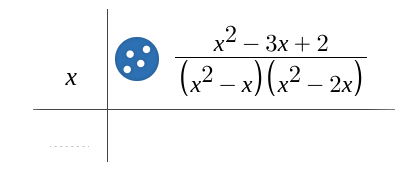
\includegraphics[width=2in]{images/desmos-limit-numerical.png}
      \end{center}
      You can enter numbers in the column titled $x$, and Desmos will show you the corresponding value of $f(x) = \dfrac{x^2 - 3x + 2}{(x^2 - x)(x^2 - 2x)}$. (Desmos will also plot the point $(x, f(x))$ on the graph.) 

      Since we're interested in evaluating $\displaystyle \lim_{x \to 2} f(x)$, we want to see what happens if $x$ is very close to \uline{but not equal to} 2. Enter several such values of $x$.

      In the table below, write down 4 of the values you entered and the corresponding values of $f(x)$; be sure to include both values that are greater than 2 and values that are greater than 2.
    \end{problem}

    \begin{problemonly}
      \begin{tabular}{p{0.5in} | p{1.5in}}
        \multicolumn{1}{c|}{$x$} & \multicolumn{1}{c}{$f(x)$} \\
        \hline
        & \\[1.5in]        
      \end{tabular}
    \end{problemonly}

    \begin{solution}
      Here's an example.
      
      \begin{tabular}{p{0.5in} | p{1.5in}}
        \multicolumn{1}{c|}{$x$} & \multicolumn{1}{c}{$f(x)$} \\
        \hline
        1.98 & 0.255 \\
        1.99 & 0.253 \\
        2.01 & 0.248 \\
        2.02 & 0.245
      \end{tabular}
    \end{solution}

    \pspace{0.25in}

  \item \label{limit-intro-numerical-guess}

    \begin{grading}
      1 point. (Since it's exploratory, full credit for any answer.) 
    \end{grading}

    \begin{problem}[\vfill\newpage]
      (Exploratory) Based on your numerical results, what do you think $\displaystyle \lim_{x \to 2} f(x)$ is? 
    \end{problem}

    \begin{solution}
      Based on our numerical results, it seems like $\lim\limits_{x \to 2} f(x) = 0.25$. 
    \end{solution}

  \item

    \begin{grading}
      3 points: 1 for simplifying the formula for $f$ algebraically, 1 for having a graph that looks like $\dfrac{1}{x^2}$, 1 for having holes at $x = 1, 2$
    \end{grading}

    \begin{problem}[\vfill]
      $f$ is a function that you know how to graph. Graph it, explaining how you got the graph. (\emph{Hint:} If you're stuck, look back at {{\#4}} in {the workbook section ``A Library of Basic Functions and Properties''}.) 
    \end{problem}

    \begin{solution}
      The function doesn't look familiar, but we can factor the numerator and denominator.
      \begin{align*}
        f(x) &= \frac{x^2 - 3x + 2}{(x^2-x)(x^2-2x)} \\
        &= \frac{(x-1)(x-2)}{x^2(x-1)(x-2)} \\
        &= \frac{1}{x^2}, x \neq 1, 2
      \end{align*}
      The graph of $y=f(x)$ will be the graph of $y=\frac{1}{x^2}$ but with holes at $x=1$ and $x=2$.

      \begin{tikzpicture}
        \begin{axis}[restrict y to domain=-3:3, xtick distance=1]
          \addplot[domain=-3:3]{1/x^2};
          \addplot[open] coordinates {(1,1) (2,0.25)};
          \node[right] at (1,1) {$(1,1)$};
          \node[above right] at (2, 0.25) {$(2,\frac{1}{4})$};
        \end{axis}
      \end{tikzpicture}
    \end{solution}

  \item

    \begin{grading}
      1 point. (Since it's exploratory, full credit for any answer.) 
    \end{grading}

    \begin{problem}[\stretch{0.4}]
      (Exploratory) Does your graph support your guess from \ref{limit-intro-numerical-guess}? Explain. 
    \end{problem}

    \begin{solution}
      Looking at the graph, as $x$ approaches $2$, $f(x)$ approaches the value $\frac{1}{4}$. This supports
      our guess that $\lim\limits_{x \to 2} f(x) = 0.25$. 
    \end{solution}

  \end{enumerate}  
\item 
{\bf Review of Quadratics:} Earlier in the semester we looked at two forms that quadratics can be written in: standard form $ax^2+bx+c$ and vertex form $a(x-h)^2+k$. In Problem 3c on this assignment, you worked with another quadratic, and analyzed its sign to determine the behavior of the second derivative. When analyzing the sign of continuous functions, we first find where the function is equal to zero and then test the sign of the function in the remaining intervals. For this reason, factoring the function to find its zeros becomes useful to us and this motivates us to explore the last form of a quadratic: {\bf factored form.}
\begin{enumerate}
    \item A quadratic written in {\bf factored form} is written $k(x-r_1)(x-r_2)$ where $r_1$ and $r_2$ are the roots or zeros of the quadratic. Rewrite the quadratic you worked with in problem 3(c) here in factored form. What are the values of $k$, $r_1$, and $r_2$ in this quadratic? (You should recycle work you did in the problem!)
    \begin{problemonly}
         \vfill
    \end{problemonly}

    \begin{solution}
        $$-3x^2 + 12 = -3(x^2-4)=-3(x+2)(x-2),$$
        so $k = -3$, $r_1 = 2$, and $r_2 = -2$.
    \end{solution}
   
    \item Not every quadratic can be factored, but many can be. Because quadratics' parabolas are symmetric, once you know the zeros, you can find the vertex, which will sit exactly between them. What is the location of the vertex (an ordered pair $(x,y)$) for the quadratic in 3(c)?
    \begin{problemonly}
         \vfill \newpage
    \end{problemonly}

    \begin{solution}
        The vertex is at $(0,12)$ as $x=0$ is directly between $-2$ and $2$. Evaluating $3x^2+12$ when $x=0$ gives us the $y-$coordinate of our vertex, and we see that this is 12. 
    \end{solution}
    
    \item Here's another quadratic $f(x)=(3-x)(x+1)$. Identify its zeros and the location of its vertex (both $x$- and $y$-coordinates). Sketch a graph of the function.
    \begin{problemonly}
         \vfill
         
    \end{problemonly}

    \begin{solution}
        The zeros for this function are at $x=3$ and $x=-1$. The location of the vertex will be at $x=1$ and we can find the $y$ coordinate by evaluating the quadratic when $x=1$. $(3-1)(1+1=4)$. The vertex is located at $(1, 4)$. Below is a graph of the function:

        \begin{tikzpicture}
      \begin{axis}[xmin=-8, xmax=8, ymin=-8, ymax=8, ytick={-8, -6, ..., 8} , grid=both,
      xtick={-8, -6, ..., 8}, xlabel=$x$, ylabel=$y$,  minor tick num=1,
      ]
    \addplot[draw=none] coordinates {(0,0)};
    \addplot[domain = -8:8, color = black]{-x^2+2*x+3};
    \end{axis}
        \end{tikzpicture}

        
    \end{solution}
    
    \item Consider the quadratic $x^2-6x+9$. Convert it to factored form and identify its zeros. What is the location of its vertex?
    \begin{problemonly}
         \vfill
    \end{problemonly}
    
    \begin{solution}
        $$x^2-6x+9=(x-3)(x-3)=(x-3)^2$$
        The function has one zero at $x=3$. The vertex will be at the location $(3,0)$. The vertex is the zero.
    \end{solution}
    \item Looking at the factored form you found in part (d), explain why the location of the vertex makes sense, given the relationship that $x^2-6x+9$ has to the parent function $x^2$ and the transformations that you can see in its formula (1-2 sentences).
    \begin{problemonly}
         \vfill
    \end{problemonly}
    
    \begin{solution}
        The factored form indicates the graph of $x^2$ has been shifted to the right by 3 units. The vertex originally located at (0,0) will now be at (3,0).
    \end{solution}
    \begin{problemonly}
         \vfill
    \end{problemonly}
\end{enumerate}
\end{enumerate}
\psreflection{For next class, read \S 7.1 - 7.3.}
\end{document}
